\chapter{}

\section{Installazione Xilnix Tool}
\label{app:a}
Al fine di effettuare tutta la creazione e riconfigurazione della zedboard tramite petalinux, dobbiamo scaricare gli opportuni tools forniti dalla Xilnix.\\
I tools necessari sono:
\begin{itemize}
\item Vivado
\item Vitis
\end{itemize}
Essi ci permettono di creare il bitstream, quindi di definire l'hardware della zedboard, al fine di far ciò scarichiamo il tutto dal sito \href{https://www.xilinx.com/support/download/index.html/content/xilinx/en/downloadNav/vivado-design-tools.html}{Xilnix}, previa registrazione, facendo attenzione alla versione di linux che si sta usando, per tutta la guida è stato usato Ubuntu 18.04.01, anche se la documentazione riferisce compatibile la versione 20.04.01(fino a .05).\\
Una volta terminata l'installazione di circa 60gb, dobbiamo importare i file inerenti alla zedboard, al fine di semplificare il lavoro di creazione del progetto. Per far ciò si seguano i seguenti passaggi:
\begin{itemize}
\item Aprire la cartella d'installazione di vivado e seguire il path
\begin{center}
\textit{path/to/vivado/version/data/boards/}
\end{center}
\item Scaricare il file \href{https://github.com/Digilent/vivado-boards/archive/master.zip}{zedboard}
\item Estrarlo in questa cartella
\end{itemize}
In questo modo avremo installato la scheda su Vivado.
\subsection{Creazione di un progetto}
\label{CreazioneVivado}
Al fine di creare il progetto sarà necessario seguire i seguenti step:
\begin{itemize}
\item Aprire vivado
\item Cliccare su "Create a new vivado project"
\item Andare avanti e dare un nome al progetto
\item Selezionare il tipo di progetto, che sara \textbf{RTL Project}
\item Inserire se esistono eventuali risorse di altri progetti già fatti in precedenza
\item Selezionare la scheda, quindi selezionare la schermata "Boards" e ricercare "zedboard"
\item Concludere la creazione
\end{itemize}
\subsection{Creazione modello}
Arrivati a questo punto dobbiamo andare a definire il nostro hardware, partendo dalla creazione dello schema, quindi creiamo un nuovo blocco 
\begin{figure}[h]
\centering
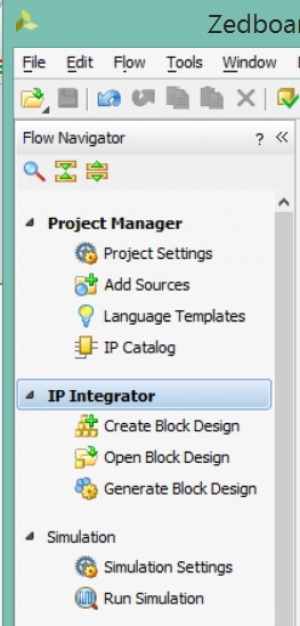
\includegraphics[width=0.2\textwidth]{images/image_7.jpg}
\end{figure}\\
Definiamo il nome e proseguiamo con la scelta dei componenti.\\
Cliccando il pulsante "Add IP" andiamo a cercare il processing system, che sarà obbligatoriamente \textbf{ZYNQ7 Processing System}.\\
Da questo punto possiamo aggiungere qualsiasi elemento di nostro interesse al fine di creare la struttura che più necessitiamo, effettuando ad ogni inserimento il comando \textit{Run Connection Automation} che ci sarà consigliato da Vivado.\\
Una volta inseriti tutti gli elementi richiesti procediamo con la rigenerazione del layout tramite il comando \verb|regenerate_bd_layout|.\\
Procediamo con le simulazioni e le sintesi al fine di poter generare il bitstream.
\subsubsection{Creazione HDL Wrapper}
L'HDL Wrapper è un file di High definition Level, che ci permette di definire il nostro progetto, tramite esso effettueremo le sintesi ed il bitstream.\\
Al fine di crearlo basterà cliccare con il tasto destro sul design creato in precedenza e cliccare la dicitura \textit{Create HDL Wrapper}
\begin{figure}[h]
\centering
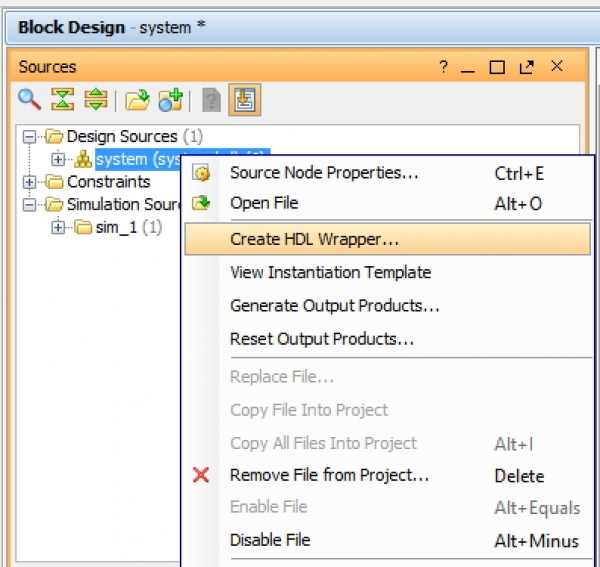
\includegraphics[width=0.4\textwidth]{images/image_20.jpg}
\end{figure}\\
\subsubsection{Sintesi}
Adesso dobbiamo avviare la sintesi, cosi da far tradurre il file HDL in una netlist\footnote{Contiene tutti i componenti che ci servono}, al fine di farla partire usiamo il pulsante \textit{Run Synthesis} che si trova nella tool bar di sinistra.
\subsubsection{Implementazione}
Questo processo mappa la sintesi che abbiamo svolto nel chip che abbiamo selezionato, nel nostro caso la zedboard. Anche qui troviamo la possibilità di far partire il tutto tramite il pulsante \textit{Run Implementation} nella tool bar di sinistra.
\subsection{Generazione del bistream}
Una volta terminati tutti questi passaggi andati a buon fine possiamo creare il file ".bit" che ci servirà più avanti per definire il kernel di petalinux. Al fine di far partire la generazione si usa il comando \textit{Generate Bitstream} presente nella tool bar di sinistra.
\subsection{Export del file di developing}\label{ExportVivado}
Al fine di creare sul nostro hardware l'immagine di petalinux, al fine di far ciò:
\begin{itemize}
\item Una volta seguiti tutti gli step precedenti clicco in alto a sinistra il pulsante file
\item Export, il terzultimo pulsante
\item Export hardware
\item Una volta aperta la finestra andiamo avanti e selezioniamo \textbf{Include bitstream}
\item Diamo un nome ed una directory ed abbiamo esportato tutto il necessario per petalinux
\end{itemize}


\chapter{}

\section{Programmazione StandAlone}
\label{Standalone}
Al fine di effettuare la programmazione StandAlone, basterà seguire i passaggi visti in precedenza fino al build del progetto, una volta che il progetto sarà buildato sarà necessario aver installati i driver della scheda.
\subsection{Installazione Driver}
Spostiamoci nella cartella d'installazione di vivado e dopodichè nel seguente path
\begin{lstlisting}
/data/xicom/cable_drivers/lin64/install_script/install_drivers/
\end{lstlisting}
da qui dovremmo semplicemente eseguire lo script.
\subsection{Flash}
Al fine di effettuare il flash sulla scheda dovremmo ritornare nel IDE, collegare la scheda nella micro USB J17, quella vicino i connettori audio, ed eseguire i seguenti passaggi:
\begin{itemize}
    \item Xilnix -> Program Device. In questa schermata che ci comparirà dobbiamo selezionare il bitstream collegato al nostro progetto e clicchiamo program.
    \item Una volta effettuato questo passaggio, clicchiamo sul progetto tasto destro \textit{Run As -> Launch Hardware}, dopodichè avremo sulla scheda ciò che abbiamo programmato.
\end{itemize}
\subsection{Collegamento Tramite UART}
Al fine di vedere il risultato a schermo della programmazione che si sta effettuando, bisogna connettersi tramite UART al connettore micro USB J14 e tramite un monitor seriale \href{https://ttssh2.osdn.jp/index.html.en}{Tera Term} su windows e tio su linux, connettersi alla scheda che solitamente sotto ambiente windows sarà COM* e sotto linux /dev/ttyACM* con un baudrate\footnote{velocità di trasmissione} di 115200, da qui potremmo interfacciarci con la scheda per usufruire del codice bare-metal che è stato caricato. \\
Questo metodo è equivalente se è presente petalinux sulla scheda.



\chapter{}

\section{Petalinux}
\label{petalinuxinst}
Per installare Petalinux, assicuriamoci che dopo l'installazione del pacchetto Vivado e Vitis restino al più 3GB.\\
Soddisfatto questo requisito, abbiamo la possibilità di percorrere due strade, l'installazione tramite self-extracting pack (una sorta di zip), ed l'installer della xilnix. Noi useremo il self-extracting pack, tanto sono equivalenti.\\
\subsection{Installazione}
Scarichiamo il file presente alla pagina \href{https://www.xilinx.com/support/download/index.html/content/xilinx/en/downloadNav/embedded-design-tools.html}{Petalinux}, se si usa una versione del sistema operativo compatibile anche l'ultima versione(2021.2) è funzionante, altrimenti usare la versione (2020.3).\\
\subsection{Requisiti}
Solitamente le dipendenze sono:
\begin{lstlisting}
sudo apt-get -y install iproute2 \
gcc \
g++ \
net-tools \
libncurses5-dev \
zlib1g:i386 \
libssl-dev \
flex \
bison \
libselinux1 \
xterm \
autoconf \
libtool \
texinfo \
zlib1g-dev \
gcc-multilib \
build-essential \
screen \
pax \
gawk \
python3 \
python3-pexpect \
python3-pip \
python3-git \
python3-jinja2 \
xz-utils \
debianutils \
iputils-ping \
libegl1-mesa \
libsdl1.2-dev \
pylint3 \
cpio
\end{lstlisting}
\subsection{Installazione}
\label{InstPeta}
Una volta scaricato il file assegnare ad esso i permessi d'esecuzione e spostarlo nella directory desiderata. Una volta effettuati questi passaggi eseguire il seguente comando:
\begin{lstlisting}
./petalinux-v<petalinux-version>-final-installer.run --dir /home/<user>/
petalinux/<petalinux-version>
\end{lstlisting}
Aggiungendo l'argomento 
\begin{lstlisting}
--platform "arm"
\end{lstlisting}
si può ridurre il peso dell'installazione a solo le zynq arm.\\
\subsection{Setup dell'ambiente lavorativo}
\label{SetupPeta}
Al fine di poter usare il tool bisogna eseguire il seguente comando:
\begin{lstlisting}
$ source <path-to-installed-PetaLinux>/settings.sh
$ source <path-to-installed-PetaLinux>/settings.csh
\end{lstlisting}
In base al tipo di Shell in cui ci troviamo.\\
Se l'output dovesse essere di questo tipo:
\begin{lstlisting}
PetaLinux environment set to '/opt/pkg/petalinux'
INFO: Checking free disk space
INFO: Checking installed tools
INFO: Checking installed development libraries
INFO: Checking network and other services
WARNING: No tftp server found - please refer to "UG1144 <petalinuxversion> PetaLinux Tools Documentation Reference Guide" for its impact
and solution
\end{lstlisting}
O al più presentare il seguente warning:
\begin{lstlisting}
WARNING: /bin/sh is not bash
\end{lstlisting}
Tutto è andato a buon fine e si può procedere con la creazione di una build.


\chapter{}
\section{Usare l'SD}
\label{sd}
\begin{itemize}
\item Formattare un SD da almeno 8GB, in due partizioni, la prima che useremo come BOOT in FAT32, con una dimensione di almeno 1GB, la seconda che useremo come root in ext4, da almeno 6GB.
\item Ora spostiamo i file :
\begin{itemize}
\item BOOT.BIN
\item image.ub, è l'immagine di linux
\item boot.scr
\end{itemize}
\item Estraiamo rootfs.tar.gz nella partizione di root
\item inseriamo l'sd nella scheda assicurandoci che sia impostata in boot da SD, quindi connettiamoci all'usb J14 e tramite un terminale seriale vediamo il boot della scheda.
\end{itemize}


\chapter{}
\section{Installazione BootGen}
\label{installazioneBoot}
Per installare bootgen è necessario usare il tool di download precedentemente scaricato in \ref{ExportVivado} e nel menu di selezione per l'installazione scegliere BOOTGEN.


\chapter{}
\section{Cross Compilazione}
\label{crossComp}
Per effettuare la cross-compilazione la strada più semplice è quella di sfruttare il cross compilatore già presente nella console di vivado, quindi per far ciò si avvii tramite shell vivado e ci si sposti nella cartella contentente il file in C, per compilare eseguire il seguente comando:
\begin{lstlisting}[language=sh, label=lst:sh, caption={Cross-compilazione}]
arm-linux-gnueabihf-gcc [nome].c -o [nome].out
\end{lstlisting}



\chapter{}
\section{Codice completo driver GPIO}
\label{GPIO}
\begin{lstlisting}[language=c, label=lst:sh, caption={Codice completo del driver GPIO}]

#include <unistd.h>
#include <time.h>
#include <stdio.h>
#include <stdlib.h>
#include <string.h>
#include <fcntl.h>
#include <sys/mman.h>
#include <sys/time.h>
#include <sys/types.h>
#include <sys/stat.h>

#define GPIO_BASE_ADDRESS       0x42000000
#define GPIO_MAP_SIZE           0x1000

#define XAXIGPIO_DATA_OFFSET    0x00000000

typedef unsigned long uint32;


int main(int argc, char *argv[]){
    unsigned long ii;
    int memfd;
    void *gpioMapAddr = NULL;

    if ( (memfd = open("/dev/mem", O_RDWR | O_DSYNC)) == -1 ){
        printf("Non riesco ad aprire /dev/mem.\n");
        exit(-1);
    }

    gpioMapAddr = mmap(0, GPIO_MAP_SIZE, PROT_READ | PROT_WRITE, MAP_SHARED, memfd, GPIO_BASE_ADDRESS);
    if (gpioMapAddr == (void *) -1){
        printf("Non posso mappare il CDMA.\n");
        exit(-1);
    }
    
    printf("GPIO mappato %p\n", gpioMapAddr);

    for(ii=0; ii<256; ii++){
        *((volatile unsigned long*) (gpioMapAddr + XAXIGPIO_DATA_OFFSET)) = ii;
        printf("led = 0x%02x\n", ii);
        usleep(20000); // sleep 20ms
    }
}

\end{lstlisting}
Qualora si volesse usare un GPIO dual channell, bisogna modificare l'offset che di default è 
$$GPIO\_BASE\_ADDRESS+ 0x08$$



\chapter{}
\section{Generazione automatica del file .bin}
\label{autoBOOT}
Al fine di effettuare la generazione automatica del file sarà necessario eseguire il seguente script, passandogli come parametri:
\begin{itemize}
    \item path/to/bitstream
    \item Architettura
    \item path/to/output
\end{itemize}
Inoltre sarà necessario creare un file \textit{template.bif} da posizionare nella stessa cartella d'esecuzione dello script
\begin{lstlisting}[language=sh, label=lst:sh, caption={Codice completo generazione automatica file BIN}]
#!/bin/bash
TMP_PATH=$(mktemp -d)
print_invalid_usage() {
	echo "Invalid usage."
	echo "Usage: generate <input_file_path> <output_directory_path>"
}
generate_bin() {
	BIT_PATH="$1"
	ARCH="$2"
	OUTPUT_PATH="$3"

	BIT_NAME=$(basename "$BIT_PATH")
	TMP_BIT_PATH="$TMP_PATH/$BIT_NAME"
	cp "$BIT_PATH" "$TMP_BIT_PATH"

	BIF_TEMPLATE_PATH="$template.bif"
	TMP_BIF_PATH="$TMP_PATH/bitstream.bif"
	sed -r "s|template.bit|$TMP_BIT_PATH|" "$BIF_TEMPLATE_PATH" > "$TMP_BIF_PATH"

	TMP_BIN_PATH="$TMP_BIT_PATH.bin"
	bootgen -image "$TMP_BIF_PATH" -arch "$ARCH" -process_bitstream bin
	if [[ $? -ne 0 ]]; then
		echo "Bin file generation failed."
		exit 1
	fi

	echo
	echo "Generating bin file..."
	BIN_PATH=$(realpath "$OUTPUT_PATH/fpga-$BIT_NAME.bin")
	cp "$TMP_BIN_PATH" "$BIN_PATH"
	echo "bin: $BIN_PATH"
}
	BIT_PATH="$1"
	ARCH="$2"
	OUTPUT_PATH="$3"

	if [[ "$BIT_PATH" = "" ]]; then
		print_invalid_usage
		exit 1
	fi

	if [[ "$OUTPUT_PATH" = "" ]]; then
		print_invalid_usage
		exit 1
	fi

	if [[ ! -f "$BIT_PATH" ]]; then
		echo "Invalid bit file path provided."
		echo "Make sure the path to the bit file is right."
		exit 1
	fi

	if [[ ! -d "$OUTPUT_PATH" ]]; then
		echo "Invalid output directory provided."
		echo "Make sure the path to the output directory is right."
		exit 1
	fi

	case "$ARCH" in	"zynq")		;;	*)
		echo "Invalid arch provided."
		exit 1
		;;
	esac

	generate_bin "$BIT_PATH" "$ARCH" "$OUTPUT_PATH"


echo
echo "Cleaning up..."
rm -rf "$TMP_PATH"

echo
echo "Finished."

\end{lstlisting}



\chapter{}
\section{Script riprogrammazione}
\label{Riprogrammazione}
Il seguente script necessita come parametri:
\begin{itemize}
    \item Il percorso fino al file binario
    \item il nome del file binario
\end{itemize}
\begin{lstlisting}[language=sh, label=lst:sh, caption={Codice completo riprogrammazione automatica FPGA}]
echo 0 > /sys/class/fpga_manager/fpga0/flags
mkdir -p /lib/firmware/
$path = $1
$nameBIN = $2
cd $path
cp $nameBIN /lib/firmware/
echo $nameBIN > /sys/class/fpga_manager/fpga0/firmware
\end{lstlisting}



